% !Tex root = dis.tex
\chapter{Likert Scale for Experimental Study}
Cognitive Code Study Code Paths Likert Scale
A Likert Scale is a psychometric scale that is commonly used in Cognitive Load Theory driven trials to gauge the subjective level of effort someone feels they need to apply to understand a given stimulus.
\begin{enumerate}
	\item Email address *

\hrulefill

	\item How hard is this code to understand? Mark only one oval.

\hspace{56pt}1 \hspace{10pt}2 \hspace{10pt}3 \hspace{10pt}4 \hspace{10pt}5 \hspace{10pt}6 \hspace{10pt}7

\hrulefill

Very easy 
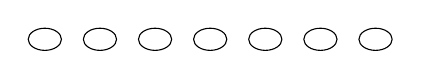
\begin{tikzpicture}
	\draw(.1,0) ellipse (6pt and 4pt);
	\draw(.8,0) ellipse (6pt and 4pt);
	\draw(1.5,0) ellipse (6pt and 4pt);
	\draw(2.2,0) ellipse (6pt and 4pt);
	\draw(2.9,0) ellipse (6pt and 4pt);
	\draw(3.6,0) ellipse (6pt and 4pt);
	\draw(4.3,0) ellipse (6pt and 4pt);
\end{tikzpicture}
Very hard

\hrulefill

	\item How hard is this code to understand? Mark only one oval.

\hspace{56pt}1 \hspace{10pt}2 \hspace{10pt}3 \hspace{10pt}4 \hspace{10pt}5 \hspace{10pt}6 \hspace{10pt}7

\hrulefill

Very easy 
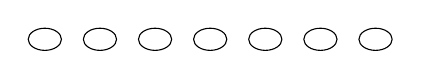
\begin{tikzpicture}
	\draw(.1,0) ellipse (6pt and 4pt);
	\draw(.8,0) ellipse (6pt and 4pt);
	\draw(1.5,0) ellipse (6pt and 4pt);
	\draw(2.2,0) ellipse (6pt and 4pt);
	\draw(2.9,0) ellipse (6pt and 4pt);
	\draw(3.6,0) ellipse (6pt and 4pt);
	\draw(4.3,0) ellipse (6pt and 4pt);
\end{tikzpicture}
Very hard

	\item How hard is this code to understand? Mark only one oval.

\hspace{56pt}1 \hspace{10pt}2 \hspace{10pt}3 \hspace{10pt}4 \hspace{10pt}5 \hspace{10pt}6 \hspace{10pt}7

\hrulefill

Very easy 
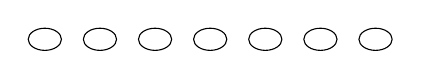
\begin{tikzpicture}
	\draw(.1,0) ellipse (6pt and 4pt);
	\draw(.8,0) ellipse (6pt and 4pt);
	\draw(1.5,0) ellipse (6pt and 4pt);
	\draw(2.2,0) ellipse (6pt and 4pt);
	\draw(2.9,0) ellipse (6pt and 4pt);
	\draw(3.6,0) ellipse (6pt and 4pt);
	\draw(4.3,0) ellipse (6pt and 4pt);
\end{tikzpicture}
Very hard

\hrulefill

	\item How hard is this code to understand? Mark only one oval.

\hspace{56pt}1 \hspace{10pt}2 \hspace{10pt}3 \hspace{10pt}4 \hspace{10pt}5 \hspace{10pt}6 \hspace{10pt}7

\hrulefill

Very easy 
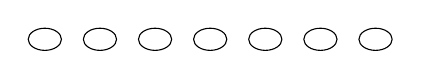
\begin{tikzpicture}
	\draw(.1,0) ellipse (6pt and 4pt);
	\draw(.8,0) ellipse (6pt and 4pt);
	\draw(1.5,0) ellipse (6pt and 4pt);
	\draw(2.2,0) ellipse (6pt and 4pt);
	\draw(2.9,0) ellipse (6pt and 4pt);
	\draw(3.6,0) ellipse (6pt and 4pt);
	\draw(4.3,0) ellipse (6pt and 4pt);
\end{tikzpicture}
Very hard

	\item How hard is this code to understand? Mark only one oval.

\hspace{56pt}1 \hspace{10pt}2 \hspace{10pt}3 \hspace{10pt}4 \hspace{10pt}5 \hspace{10pt}6 \hspace{10pt}7

\hrulefill

Very easy 
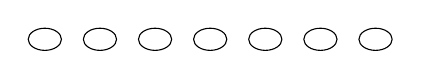
\begin{tikzpicture}
	\draw(.1,0) ellipse (6pt and 4pt);
	\draw(.8,0) ellipse (6pt and 4pt);
	\draw(1.5,0) ellipse (6pt and 4pt);
	\draw(2.2,0) ellipse (6pt and 4pt);
	\draw(2.9,0) ellipse (6pt and 4pt);
	\draw(3.6,0) ellipse (6pt and 4pt);
	\draw(4.3,0) ellipse (6pt and 4pt);
\end{tikzpicture}
Very hard

\hrulefill

	\item How hard is this code to understand? Mark only one oval.

\hspace{56pt}1 \hspace{10pt}2 \hspace{10pt}3 \hspace{10pt}4 \hspace{10pt}5 \hspace{10pt}6 \hspace{10pt}7

\hrulefill

Very easy 
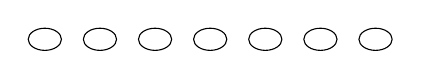
\begin{tikzpicture}
	\draw(.1,0) ellipse (6pt and 4pt);
	\draw(.8,0) ellipse (6pt and 4pt);
	\draw(1.5,0) ellipse (6pt and 4pt);
	\draw(2.2,0) ellipse (6pt and 4pt);
	\draw(2.9,0) ellipse (6pt and 4pt);
	\draw(3.6,0) ellipse (6pt and 4pt);
	\draw(4.3,0) ellipse (6pt and 4pt);
\end{tikzpicture}
Very hard

	\item How hard is this code to understand? Mark only one oval.

\hspace{56pt}1 \hspace{10pt}2 \hspace{10pt}3 \hspace{10pt}4 \hspace{10pt}5 \hspace{10pt}6 \hspace{10pt}7

\hrulefill

Very easy 
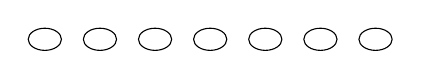
\begin{tikzpicture}
	\draw(.1,0) ellipse (6pt and 4pt);
	\draw(.8,0) ellipse (6pt and 4pt);
	\draw(1.5,0) ellipse (6pt and 4pt);
	\draw(2.2,0) ellipse (6pt and 4pt);
	\draw(2.9,0) ellipse (6pt and 4pt);
	\draw(3.6,0) ellipse (6pt and 4pt);
	\draw(4.3,0) ellipse (6pt and 4pt);
\end{tikzpicture}
Very hard

\hrulefill

	\item How hard is this code to understand? Mark only one oval.

\hspace{56pt}1 \hspace{10pt}2 \hspace{10pt}3 \hspace{10pt}4 \hspace{10pt}5 \hspace{10pt}6 \hspace{10pt}7

\hrulefill

Very easy 
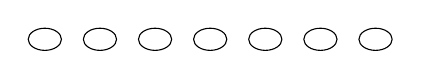
\begin{tikzpicture}
	\draw(.1,0) ellipse (6pt and 4pt);
	\draw(.8,0) ellipse (6pt and 4pt);
	\draw(1.5,0) ellipse (6pt and 4pt);
	\draw(2.2,0) ellipse (6pt and 4pt);
	\draw(2.9,0) ellipse (6pt and 4pt);
	\draw(3.6,0) ellipse (6pt and 4pt);
	\draw(4.3,0) ellipse (6pt and 4pt);
\end{tikzpicture}
Very hard

	\item How hard is this code to understand? Mark only one oval.

\hspace{56pt}1 \hspace{10pt}2 \hspace{10pt}3 \hspace{10pt}4 \hspace{10pt}5 \hspace{10pt}6 \hspace{10pt}7

\hrulefill

Very easy 
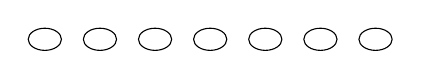
\begin{tikzpicture}
	\draw(.1,0) ellipse (6pt and 4pt);
	\draw(.8,0) ellipse (6pt and 4pt);
	\draw(1.5,0) ellipse (6pt and 4pt);
	\draw(2.2,0) ellipse (6pt and 4pt);
	\draw(2.9,0) ellipse (6pt and 4pt);
	\draw(3.6,0) ellipse (6pt and 4pt);
	\draw(4.3,0) ellipse (6pt and 4pt);
\end{tikzpicture}
Very hard

\hrulefill

	\item How hard is this code to understand? Mark only one oval.

\hspace{56pt}1 \hspace{10pt}2 \hspace{10pt}3 \hspace{10pt}4 \hspace{10pt}5 \hspace{10pt}6 \hspace{10pt}7

\hrulefill

Very easy 
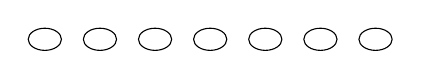
\begin{tikzpicture}
	\draw(.1,0) ellipse (6pt and 4pt);
	\draw(.8,0) ellipse (6pt and 4pt);
	\draw(1.5,0) ellipse (6pt and 4pt);
	\draw(2.2,0) ellipse (6pt and 4pt);
	\draw(2.9,0) ellipse (6pt and 4pt);
	\draw(3.6,0) ellipse (6pt and 4pt);
	\draw(4.3,0) ellipse (6pt and 4pt);
\end{tikzpicture}
Very hard

	\item How hard is this code to understand? Mark only one oval.

\hspace{56pt}1 \hspace{10pt}2 \hspace{10pt}3 \hspace{10pt}4 \hspace{10pt}5 \hspace{10pt}6 \hspace{10pt}7

\hrulefill

Very easy 
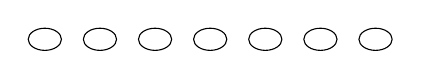
\begin{tikzpicture}
	\draw(.1,0) ellipse (6pt and 4pt);
	\draw(.8,0) ellipse (6pt and 4pt);
	\draw(1.5,0) ellipse (6pt and 4pt);
	\draw(2.2,0) ellipse (6pt and 4pt);
	\draw(2.9,0) ellipse (6pt and 4pt);
	\draw(3.6,0) ellipse (6pt and 4pt);
	\draw(4.3,0) ellipse (6pt and 4pt);
\end{tikzpicture}
Very hard

\hrulefill

	\item How hard is this code to understand? Mark only one oval.

\hspace{56pt}1 \hspace{10pt}2 \hspace{10pt}3 \hspace{10pt}4 \hspace{10pt}5 \hspace{10pt}6 \hspace{10pt}7

\hrulefill

Very easy 
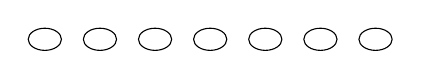
\begin{tikzpicture}
	\draw(.1,0) ellipse (6pt and 4pt);
	\draw(.8,0) ellipse (6pt and 4pt);
	\draw(1.5,0) ellipse (6pt and 4pt);
	\draw(2.2,0) ellipse (6pt and 4pt);
	\draw(2.9,0) ellipse (6pt and 4pt);
	\draw(3.6,0) ellipse (6pt and 4pt);
	\draw(4.3,0) ellipse (6pt and 4pt);
\end{tikzpicture}
Very hard

	\item How hard is this code to understand? Mark only one oval.

\hspace{56pt}1 \hspace{10pt}2 \hspace{10pt}3 \hspace{10pt}4 \hspace{10pt}5 \hspace{10pt}6 \hspace{10pt}7

\hrulefill

Very easy 
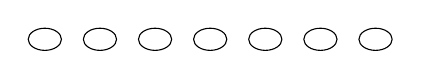
\begin{tikzpicture}
	\draw(.1,0) ellipse (6pt and 4pt);
	\draw(.8,0) ellipse (6pt and 4pt);
	\draw(1.5,0) ellipse (6pt and 4pt);
	\draw(2.2,0) ellipse (6pt and 4pt);
	\draw(2.9,0) ellipse (6pt and 4pt);
	\draw(3.6,0) ellipse (6pt and 4pt);
	\draw(4.3,0) ellipse (6pt and 4pt);
\end{tikzpicture}
Very hard

\hrulefill

	\item How hard is this code to understand? Mark only one oval.

\hspace{56pt}1 \hspace{10pt}2 \hspace{10pt}3 \hspace{10pt}4 \hspace{10pt}5 \hspace{10pt}6 \hspace{10pt}7

\hrulefill

Very easy 
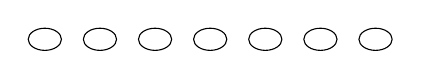
\begin{tikzpicture}
	\draw(.1,0) ellipse (6pt and 4pt);
	\draw(.8,0) ellipse (6pt and 4pt);
	\draw(1.5,0) ellipse (6pt and 4pt);
	\draw(2.2,0) ellipse (6pt and 4pt);
	\draw(2.9,0) ellipse (6pt and 4pt);
	\draw(3.6,0) ellipse (6pt and 4pt);
	\draw(4.3,0) ellipse (6pt and 4pt);
\end{tikzpicture}
Very hard

	\item How hard is this code to understand? Mark only one oval.

\hspace{56pt}1 \hspace{10pt}2 \hspace{10pt}3 \hspace{10pt}4 \hspace{10pt}5 \hspace{10pt}6 \hspace{10pt}7

\hrulefill

Very easy 
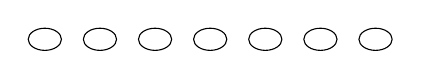
\begin{tikzpicture}
	\draw(.1,0) ellipse (6pt and 4pt);
	\draw(.8,0) ellipse (6pt and 4pt);
	\draw(1.5,0) ellipse (6pt and 4pt);
	\draw(2.2,0) ellipse (6pt and 4pt);
	\draw(2.9,0) ellipse (6pt and 4pt);
	\draw(3.6,0) ellipse (6pt and 4pt);
	\draw(4.3,0) ellipse (6pt and 4pt);
\end{tikzpicture}
Very hard

\hrulefill

	\item How hard is this code to understand? Mark only one oval.

\hspace{56pt}1 \hspace{10pt}2 \hspace{10pt}3 \hspace{10pt}4 \hspace{10pt}5 \hspace{10pt}6 \hspace{10pt}7

\hrulefill

Very easy 
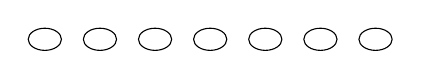
\begin{tikzpicture}
	\draw(.1,0) ellipse (6pt and 4pt);
	\draw(.8,0) ellipse (6pt and 4pt);
	\draw(1.5,0) ellipse (6pt and 4pt);
	\draw(2.2,0) ellipse (6pt and 4pt);
	\draw(2.9,0) ellipse (6pt and 4pt);
	\draw(3.6,0) ellipse (6pt and 4pt);
	\draw(4.3,0) ellipse (6pt and 4pt);
\end{tikzpicture}
Very hard

	\item How hard is this code to understand? Mark only one oval.

\hspace{56pt}1 \hspace{10pt}2 \hspace{10pt}3 \hspace{10pt}4 \hspace{10pt}5 \hspace{10pt}6 \hspace{10pt}7

\hrulefill

Very easy 
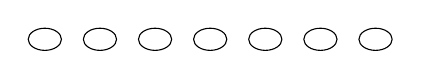
\begin{tikzpicture}
	\draw(.1,0) ellipse (6pt and 4pt);
	\draw(.8,0) ellipse (6pt and 4pt);
	\draw(1.5,0) ellipse (6pt and 4pt);
	\draw(2.2,0) ellipse (6pt and 4pt);
	\draw(2.9,0) ellipse (6pt and 4pt);
	\draw(3.6,0) ellipse (6pt and 4pt);
	\draw(4.3,0) ellipse (6pt and 4pt);
\end{tikzpicture}
Very hard
\end{enumerate}